\documentclass[11pt, oneside]{article}   	% use "amsart" instead of "article" for AMSLaTeX format
\usepackage{geometry}                		% See geometry.pdf to learn the layout options. There are lots.
\geometry{a4paper}                   		% ... or a4paper or a5paper or ... 
\usepackage{graphicx}
\title{Slides 01}
%\date{}							% Activate to display a given date or no date
\usepackage{amsmath}

\begin{document}
\maketitle
\section{Introduction}
What is an encryption scheme? A triplet  $<Gen,Enc,Dec>.$
\begin{enumerate}
\item Gen: Probabilistically selects a key k
\item Enc: Encrypts message m with key k $c := Enc_k(m)$
\item Dec: Decrypts ciphertext c with key k as $m := Dec_k(c)$
\end{enumerate}
\emph{The same key is used for Enc and Dec, symmetric/private-key encryption.}
\begin{figure}[ht]
    \centering
    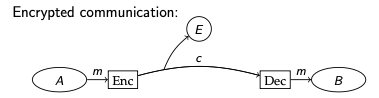
\includegraphics[width=6cm]{figures/f1.png}
    \caption{Basic Communication}
\end{figure}
\subsection{Cryptanalysis}
Cryptanalysis: The art of code breaking/cracking
\subsubsection{Kerckhoffs' principle}
Only the key should be secret in an encryption scheme. Why?
\begin{itemize}
\item A key is easier to exchange secretly than a full system
\item In case of compromise, the key is easier to update
\item Encryption scheme can be reused
\item It allows public algorithms to be scrutinised, and standardised.
\end{itemize}
\subsubsection{Attacker model}
Depending on the context:
\begin{enumerate}
\item Passive:
	\begin{itemize}
	\item Ciphertext-only: you only see ciphertexts
	\item Known-plaintext: you see some plaintext/ciphertext pairs
	\end{itemize}
\item Active:
	\begin{itemize}
	\item Chosen-plaintext: you can ask for the encryption of some messages
	\item  Chosen-ciphertext: you can also ask for the decryption of some ciphertexts 
	\end{itemize}
\end{enumerate}
\subsubsection{Lessons}
\begin{enumerate}
\item Key space should not be explorable when messages are long. In practice trying all possible keys should require at least $2^{80}$ computational steps. \\
\emph{Improvement on Ceaser's Cipher}, since we could have tried all possible 26 keys and get the message. Now not just a shift but take any permutation of the alphabet. This is $26! \approx 2^{88} keys$.
How do we break it though? It is still possible, if you know the plaintext language, frequency analysis is possible.
\item Large key space is not enough!
\item We need something secure \emph{independently of the message distribution}.\\
\emph{Another improvement on Ceaser's Cipher}, instead of a constant shift, use different shifts according to position. A key is a sequence of numbers in $[0,25]$. Breaking is still possible, if you have enough ciphertext material, you can make quesses on the key length and then make frequency analysis.
\item We can keep going with other tricks but there are other things we can consider ...
\end{enumerate}

\section{Modern Cryptography}
\subsection{Definitions}
\begin{enumerate}
\item What do we want to do?
\item Shall I use this scheme here?
\item Why choosing this scheme rather than that one?
\end{enumerate}
\newpage
What should the definition of security say for an encryption scheme?
\begin{enumerate}
\item Given any ciphertext, no adversary should be able to recover the key
\item Given any ciphertext, no adversary should be able to recover the plaintext
\item Given any ciphertext, no adversary should be able to recover any character of the plaintext
\item Given any ciphertext, no adversary should be able to recover any function of the plaintext
\end{enumerate}

In modern cryptography, most schemes rely on computational assumptions. We should be able to relate the schemes and definitions to assumptions. \\
$=>$ Reductionist approach: if someone can break this scheme, then my assumption can be falsified.
\subsubsection{Perfect encryption}
\begin{quote}
Perfect encryption is possible (Shannon, 1949)
\end{quote}
Again, what is an encryption scheme? A triplet $<Gen, Enc, Dec>$.
\begin{enumerate}
\item Gen: Probabilistically selects a key $k \in \mathcal{K}$
\item Enc: Encrypts message $m \in \mathcal{M}$ with key k $c \leftarrow Enc_k(m)$
\item Dec: Decrypts ciphertext $c \in \mathcal{C}$ with key k as $m := Dec_k(c)$
\end{enumerate}
Remarks:
\begin{itemize}
\item Enc may be probabilistic (it is most of the time)
\item $Dec_k(Enc_k(m))=m$, always. So assume, Dec to be deterministic.
\item Assume $|\mathcal{M}| > 1$
\item Assume $\mathcal{M}$ and $\mathcal{C}$ only contain messages and ciphertexts that may happen.
\end{itemize}
\emph{Definition:} $<Gen, Enc, Dec>$ over message space $\mathcal{M}$ is perfectly secret if, for every probability distribution over $\mathcal{M}$, every message $m \in \mathcal{M}$, and every ciphertext $c \in \mathcal{C}$:
\begin{equation}
Pr[M=m|C=c] = Pr[M=m]
\end{equation}
In other words, this means that given the ciphertext you know nothing about the message. So, it is impossible to distinguish the ciphertext corresponding to two plaintexts.\\
\emph{Equivalent Definition:} $<Gen, Enc, Dec>$ over message space $\mathcal{M}$ is perfectly secret if, for every probability distribution over $\mathcal{M}$, every message $m \in \mathcal{M}$, and every ciphertext $c \in \mathcal{C}$:
\begin{equation}
Pr[C=c|M=m] = Pr[C=c]
\end{equation}
\emph{Proof of Equivalence:} Using Bayes
\begin{equation}
Pr[C=c|M=m] = \frac{Pr[M=m|C=c] \cdot Pr[C=c]}{Pr[M=m]} = Pr[C=c]
\end{equation}
Rearranging the above gives equation 1.\\
\\
\\
\textbf{Experiment} $Priv_{\mathcal{A},\prod}^{eav}$

\begin{enumerate}
\item $\mathcal{A}$ outputs $m_0,m_1 \in \mathcal{M}$
\item Choose $k \leftarrow \mathcal{K}$ and  $b \leftarrow {0,1}$ and send $Enc_k(m_b)$ to $\mathcal{A}$
 \item $\mathcal{A}$ outputs $b'$
 \item Define $Priv_{\mathcal{A},\prod}^{eav}:=1$ iff $b=b'$
\end{enumerate}

Over the message space $\mathcal{M}$, $\prod=<Gen,Enc,Dec>$ is perfectly secret if for every adversary $\mathcal{A}$:
\begin{equation}
Pr[Priv_{\mathcal{A},\prod}^{eav}:=1] = \frac{1}{2}
\end{equation}
Interpretation: Even if $\mathcal{A}$ chooses 2 messages, it cannot decide which of them has been encrypted.
\subsubsection{One-time pad}
One-time pad is perfectly secret!
\begin{itemize}
\item Fix $ l> 0$. $\mathcal{M}=\mathcal{K}=\mathcal{C}={0,1}^{l}$
\item $Gen$ selects uniformly in $\mathcal{K}$
\item $Enc_k(m) := m \oplus k$
\item $Dec_k(c) := c \oplus k$
\end{itemize}
\emph{Proof:} Fix any distribution over $\mathcal{M}$, any $m \in \mathcal{M}$ and $c \in \mathcal{C}$.
\begin{equation}
\begin{aligned}
    \Pr[ C=c \,|\,  M=m] &= \Pr[M \oplus K = c \, | \, M = m] \\
    &= \Pr[m \oplus K =c ]\\
    &= Pr[K=m\oplus c] = \frac{1}{2^l}\\
    &= Pr[C=c \,|\,M=m'] \text{ for every } m'
\end{aligned}
\end{equation}
One time pad is not convenient to use:
\begin{itemize}
\item Key needs to be as long as the message!
\item Suppose $m,m'$ is encrypted with $k$
\begin{equation}
(m\oplus k) \oplus (m'\oplus k) = m \oplus m'
\end{equation}
$\mathcal{A}$ wins if it can play $Priv_{\mathcal{A},\prod}^{eav}$ twice with the same key!
\end{itemize}
\subsubsection{Limits of perfect secrecy}
Suppose $\prod:=<Gen,Enc,Dec>$ is s.t. $|\mathcal{K}| < |\mathcal{M}|$ (meaning, the key space is smaller than the message space, not as many keys as messages). Then $\prod$ is not a perfectly secret encryption scheme.\\
\emph{Proof:} Consider uniform distribution on $\mathcal{M}$ and any $c \in \mathcal{C}$\\
Define $\mathcal{M}(c):=\{m\,:\,c=Enc_k(m) \text{ for some } k \in \mathcal{K}\}$\\
We have $|\mathcal{M}(c)| \le |\mathcal{K} < |\mathcal{M}|$\\
Therefore, $\exists m^* \in \mathcal{M} - \mathcal{M}(c)$, and
\begin{equation}
Pr[M=m^*\,|\,C=c]=0 \neq \frac{1}{|\mathcal{M}|} = Pr[M=m^*]
\end{equation}
This is a problem in the context of perfect secrecy. In a perfectly secret encryption scheme, having the ciphertext should provide no additional information about the plaintext. But here, the fact that $Pr[M=m^*|C=c]=0$ implies that given the ciphertext, you can be certain that the plaintext is not $m^*$, which violates the perfect secrecy condition.\\
\textbf{Conclusion}: Perfectly secret encryption schemes exist, but they are difficult to use.

















\end{document}  